\documentclass[sigconf,anonymous=true]{acmart}

\usepackage{booktabs} % For formal tables

% Copyright
%\setcopyright{none}
%\setcopyright{acmcopyright}
%\setcopyright{acmlicensed}
\setcopyright{rightsretained}
%\setcopyright{usgov}
%\setcopyright{usgovmixed}
%\setcopyright{cagov}
%\setcopyright{cagovmixed}

\settopmatter{printacmref=true}



% DOI
\acmDOI{10.475/123_4}

% ISBN
\acmISBN{123-4567-24-567/08/06}

%Conference
\acmConference[WOODSTOCK'18]{ACSAC conference}{April 2018}{El
  Paso, Texas USA}
\acmYear{2018}
\copyrightyear{2018}

\acmArticle{4}
\acmPrice{15.00}

% These commands are optional
%\acmBooktitle{Transactions of the ACM Woodstock conference}
\editor{Jennifer B. Sartor}
\editor{Theo D'Hondt}
\editor{Wolfgang De Meuter}


\begin{document}
\title{Anti-Methods for Distributed Web-Crawler}
\titlenote{Produces the permission block, and
  copyright information}

\author{In Woo Ro}
\authornote{Dr.~Trovato insisted his name be first.}
\orcid{1234-5678-9012}
\affiliation{%
  \institution{Hanyang University}
  \streetaddress{P.O. Box 1212}
  \city{Seoul}
  \country{Korea}
  \postcode{43017-6221}
}
\email{inwoo13@hanyang.ac.kr}

\author{Joong Soo Han}
\authornote{The secretary disavows any knowledge of this author's actions.}
\affiliation{%
  \institution{Hanyang University}
  \city{Seoul}
  \country{Korea}
  \postcode{43017-6221}
}
\email{soohan@hanyang.ac.kr}

\author{Eul Gyu Im}
\authornote{This author is the
  one who did all the really hard work.}
\affiliation{%
  \institution{Hanyang University}
  \city{Seoul}
  \country{Korea}
  \postcode{43017-6221}
  }
\email{imeg@hanyang.ac.kr}

% The default list of authors is too long for headers.
\renewcommand{\shortauthors}{B. Trovato et al.}


\begin{abstract}
In this paper, we propose node reducing as a countermeasure against distributed crawlers.\footnote{This is an abstract footnote}
\end{abstract}


\keywords{Web Crawler, Traffic Analysis}

\maketitle

%
% Introduction
%
\section{Introduction}
Data utilization and analysis are no longer the domain of data mining or analysts, and it has become a fundamental skill from students to researchers. 
In order to utilize the data, it is necessary to retain the data first, but the required data does not always exist in the form of the completed data set. Therefore, in many cases, you need to collect the data you need through web crawling.
There are two problems. One is that web service data distribution method can be changed through updating (crawler must be updated to reflect the structure change of input data), and the other is to introduce anti-crawling method in some web services the crawler will spend a lot of time developing the crawler.
In this paper, we introduce the anti-crawling methods and its countermeasures, and show that the conventional anti - crawling method cannot defend the distributed crawler. We also introduce a new anti-crawling technique that gradually adds an IP set using a distributed crawler to the black-list.



%
% Back Ground
% with 2 subsections
%
\section{Back Ground}
\begin{enumerate}
\item Http Archive
\newline Http Archive is a file format that stores network logs obtained through a built-in developer tool for web browsers such as Internet Explorer and Chrome. Network logs are stored as a .har extension files with JSON format. The HAR file consists of metadata about the log itself and entries data for request and response contents. Metadata includes information such as browser type, version, and creation time. In the entries section, start time, time required, and request and response data are included for each entry.
The request and response items in the entry contain all the data that can be found through the developer tool. This means that the developer can obtain the same amount of information as the real-time monitoring of the actual site behavior by checking the har logs. Furthermore, by parsing the har logs, the data necessary for crawler development is automatically extracted.
\newline
\item Power Law
\newline 
According to the rule of thumb, when the items are sorted in order of frequency of use, the frequency of use decreases exponentially every time the rank decreases. This is also common for web traffic, and most web traffic is focused on some frequently used items. In this paper, we also introduce a technique for identifying crawler sets using items in the long-tail region, assuming that web traffic follows the power law.
\end{enumerate}



%
% GENERATING CRAWLING LIBRARY:HAR2LIB
% with 2 subsections
%
\section{Generating Crawling Library:HAR2LIB}
In this chapter, we introduce the har2lib package which generates the crawling library code by parsing the har log file as an example of Intelligent Crawler.

\subsection{Parsing HAR Files}
HAR2LIB provides the harlib class. When you create a class object, it loads the har log file and then parses it. Parsing can be divided into exception handling, header analysis, and URL analysis.

\subsection{Generating Crawling Library}
When parsing is complete, HAR2LIB calls the internal \newline\verb|harlib._gen_py()| method to create a python class that contains a crawling method for the site. Next, the request header information is stored in a dict form inside the method so that the HTTP header can be set to be the same as that transmitted from the browser. The generated class will only contain the necessary methods for crawling, and actually implement the business logic that calls it. This is because the crawling data coding part and the crawling scenario implementation part are separate issues.



%
% ANTI-CRAWLING METHODS AND COUNTER SCENARIO
% with 2 subsections
%
\section{ANTI-CRAWLING METHODS AND COUNTER SCENARIO}
Although Harlib does not present the crawling scenario directly, there are features that help create a crawling scenario, such as an automated dealy. In this chapter, we introduce the anti-crawling technique to detect and respond to the crawler and the bypassing technique.

\subsection{Anti-Crawling Methods}
Detecting crawlers that perform excessive crawling on Web services and performing blocking automatically are very important for service management and intellectual property protection. This section introduces the known anti-crawling techniques.



\begin{enumerate}
\item HTTP Header Check
\newline For a typical crawler, do not use the http header used by the browser. The server distinguishes the normal user from the crawler by checking the request header from the client and checking whether the value of User-Agent is normally included.
\newline
\item Access Frequency Recognition
\newline 
An attacker performing an aggressive crawling predefines the core data that the web service wants to collect, and implements a crawler that requests specific data without requesting unnecessary resources. In this case, the web server must process only a large number of consecutive calls to specific resources. For example, suppose you are an attacker attempting to replicate all the data of a Web service that has real estate transfer data for 5.6 million copies in Korea. When the web service retrieves the lot number, it passes the html, js, and css files to the client and dynamically completes the data that fills the html table form with ajax call. The attacker can implement only the ajax call with a script such as python, and obtain the data from the public address list and request data to the server in parallel. If you are a careful attacker, you will not get close to the performance limit of the server, but if not, you will parallelize the collection process to get the data you want as soon as possible.
\newline
\item Access Pattern Recognition
\newline
Access pattern recognition is an anti-crawling method through dynamic analysis in addition to the above access frequency recognition. If a client requests only a specific resource continuously without a call to a resource that should normally be requested, the corresponding IP is blocked. In the case of a web service using advanced approach to access pattern recognition, the service is viewed as a set of consecutive requests from the viewpoint of the user UX, and requests and responses belonging to the same set are chained by including a specific hash value in the cookie. Some requests can not be made separately.
\end{enumerate}


\subsection{Anti-Cralwer Counter Method}
When using the intelligent Crawler library created through har2lib described in the previous chapter 3, the following three anti-crawling methods can be used as follows. The distributed crawler using all of the techniques 1 to 3 can not be defended by the anti-crawling technique described above.



\begin{enumerate}
\item Request Header Replay
\newline All request methods generated by har2lib automatically mount the same http request header as requested by a normal browser. Web services can not distinguish between crawlers and browsers with http header verifications.
\newline
\item Access Frequency Auto Configuration
\newline 
har2lib sets the automated dealy time value for each method using the actual time data for each method in the har parsing process. All methods manipulate the delay, which is actually taken, through the sleep function when the auto dealy option is set to True. After the configuration is applied, it is possible to configure a parallel crawling network consisting of units that do not exceed the access frequency limit per IP when combined with multiple IP proxy servers.
\newline
\item Access Pattern Replay
\newline
Although har2lib does not write the crawling scenario directly, it supports a guide to the access pattern that helps scenarios that only replicate the ajax call clone to bypass the approach pattern. Since the harlog itself records normal access patterns, it is possible to summarize the access patterns in a separate chart.
\end{enumerate}



%
% BLOCKING DISTRIBUTED CRAWLER
% with 2 subsections
%
\section{BLOCKING DISTRIBUTED CRAWLER}
In this section, we propose a new technique to detect and block distributed crawlers that could not be defended by existing anti-crawling techniques.

\subsection{Number of Distributed Nodes}
In order for the Distributed crawler to replicate the historical data of a website, the following conditions must be met. Cn ≥ Um / (Td * 30) for the number of items (Um) updated in the target site on a month, the maximum number of connections (Td) per day restricted by the site, and the number of IPs (Cn) Must be satisfied.
For example, if a service that updates 60,000 data per month limits the maximum number of connections per day to 50, an attacker must perform crawling using at least 40 distributed IPs. Conversely, on the service provider side, the larger the Um, the smaller the Td is, the more advantageous it is. However, Um is difficult to secure arbitrarily, and if Td is reduced, the ratio of false positives to normal users increases.


\subsection{Node Reducing with statistical approach}
Instead of increasing the Um from the service provider side, or reducing the Td is a method of identifying a portion of the crawler to Cn and Cn by reducing the block.
Assuming that the number of IPs used by the attacker is Cm, the attacker must satisfy Cn - Cm ≥ Um / (Td * 30). On the service provider side, Cm satisfying Cm ≥ Cn - Um / (Td * 30) can be obtained.
Service providers can create a block-list without reducing Td in a batch by using statistical techniques. The frequency of access by users is not the same for each item, and when the items with the highest frequency of access are arranged on the left side, they are distributed in a graph form which exponentially decreases according to a power law as follows.

\begin{figure}[H]
    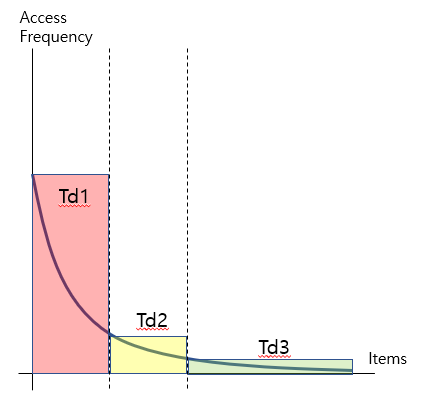
\includegraphics[width=1.0\columnwidth]{figs/figure_01.png}
    \caption{Access Frequency per number of connections}
    \label{fig:my_label}
\end{figure}

In order for an attacker to replicate historical data from the service, he must also access the items in the long-tail (Td3) interval. However, the attacker does not know exactly which item the item he is accessing belongs to. Using this information asymmetry, service providers can easily identify IPs that are accessed more frequently than long-tailed segments. If we start to increase the Cm value through the long-tail interval, the attacker will crawl with a smaller number of IPs, and Cm will increase in the Td2 interval.
The Td value for each interval is calculated by adding the standard deviation (s) of the corresponding interval access frequency to the access frequency value (Amax) of the item having the highest access frequency per IP among the corresponding interval items as follows. 

  \begin{displaymath}
    Td = Amax + s * 2
  \end{displaymath}

If a particular IP accesses an item in the long-tail region with more than the Td value determined by the above formula, it can be included in the block-list.

\subsection{Dummy Items}
The service provider may include a dummy item to detect the crawler in addition to the actual service target item. The item is normally inaccessible to the general user through the UI. For example, it exists as an HTML tag but it is not displayed on the screen due to the attribute setting or the case where the ordinary user is not interested because it exists on the index but is not in the real world.
Such a dummy item may approach a crawler that performs sequential access but it can maintain a relatively low threshold value because the accessibility of the general user is low and it generates a lower interval than the long-tail interval derived from the traffic can do.



%
% EXPERIMENT
%
\section{EXPERIMENT}
In order to verify the above, experiments were performed to classify the crawler IP for the actual web traffic data. It is based on the web traffic of 1 month released by NASA. Details and experimental method of data are as follows.


\subsection{Web Traffic Data}


\begin{enumerate}
\item Source
\newline NASA released a total of 1,891,715 access logs for the month of July 1995. In this paper, the log is parsed into csv format and composed of 4 columns including IP, date, access target and access result.
The total number of connected IPs is 81,978 and the number of items is 21,649. The most accessed items received 111,116 requests as '/images/NASA-logosmall.gif'.
\newline
\item Traffic Distribution
\newline 
The total number of accesses is calculated for each access target, and the sorting is performed in order of the largest number of connections. The results are confirmed to be distributed in a form in which a power law is applied as described in Section 5. 
In addition, as shown in Figures 2, 3 and 4, power distribution is also observed internally in Td1, Td2, and Long-tail sections. Figurue 2 is a graph of connection frequency of 38 items corresponding to the upper 0.5\% of Td1, Figure 3 shows the top 100 ~ 2000 figures corresponding to Td2, Figure 4 shows the frequency of 100 ~ 2000 . In the next section of the simulator, node reduction will be performed using a set of items belonging to the long-tail as described above.
\end{enumerate}

\begin{figure}[H]
    \centering
    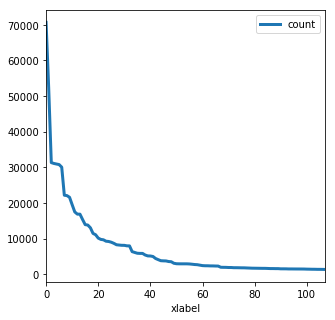
\includegraphics[width=0.7\columnwidth]{figs/figure_02_td1.png}
    \caption{Access Count in Td1}
    \label{fig:my_label}
\end{figure}

\begin{figure}[H]
    \centering
    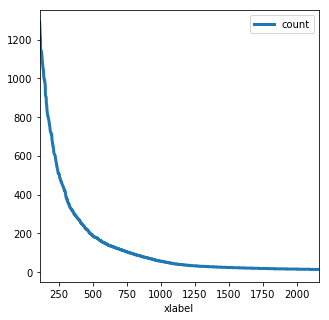
\includegraphics[width=0.7\columnwidth]{figs/figure_03_td2.png}
    \caption{Access Count in Td2}
    \label{fig:my_label}
\end{figure}

\begin{figure}[H]
    \centering
    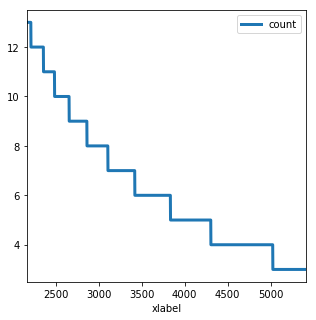
\includegraphics[width=0.7\columnwidth]{figs/figure_04_td3.png}
    \caption{Access Count in Long-tail}
    \label{fig:my_label}
\end{figure}

\subsection{Simulation}
In this paper, we implemented two kinds of simulation. One is to check whether it is possible to detect and disable the crawler IP group by performing node reduction through items belonging to the long-tail, and the other is to check false positive when the actual traffic is input to the same detection logic .


\begin{enumerate}
\item Data Pre-Processing
\newline In order to prevent duplication of data used in modeling and experimental data in the time series data, Long-tail was constructed by using data from 1 to 24 days in 30 matching data. Traffic verification was performed from the 25th to the last day Data. \& Lt; / RTI \& gt;
When accessing html files, gif extension files are removed from the long-tail group in order to prevent cumulative access values from increasing in duplicate while accessing gif extension files together.
Finally, the request log which was not accessed successfully was excluded from the experiment.
\newline
\item Simulators
\newline 
The simulator is implemented using python. The parameters are the size of the distributed IP set used by the crawler, the long-tail list, the entire item list, and threshold values used for detection.
The implementation method allows the Crawler IP Set to access each item by traversing the entire item list, and accesses the IP in the crawler distributed IP set at each access.
When the crawler accesses a long-tail entry, it adds the IP to the warning dictionary and increments the access count by one. However, if the same IP accesses the same item, it does not increase the access count because it is not related to the purpose of crawling. When the access count exceeds the threshold value, Node Reducing is implemented by adding the corresponding IP to the banned list. Figure 5 below shows an example of running a crawler using 100 distributed IPs for 7,649 items. The number of long-tail items is 5,355 and the threshold is set to 20. 

\begin{figure}[H]
    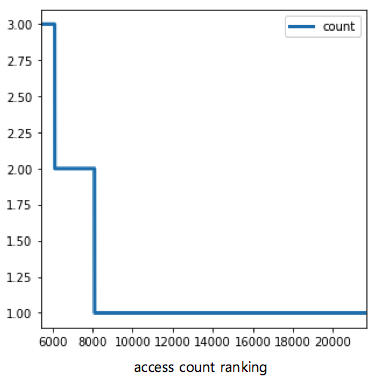
\includegraphics[width=0.65\columnwidth]{figs/figure_05_td4.png}
    \caption{Number of IPs using crawling}
    \label{fig:my_label}
\end{figure}

The IPs included in the crawler IP set gradually accumulate the access count, and the node reduction starts from the point when the access count of the entire crawler node group increases beyond {number of nodes} * {threshold}.
Another function of the simulator is to input the request request to the crawler simulator based on the actual web traffic log. This is implemented to confirm the case where the simulator judges the actual web traffic as a crawler.
\newline
\item Node Reducing Result
\newline 
Experiments were performed with threshold set to 30, and the crawler set consisting of up to 222 nodes was completely detectable. If the number of nodes exceeded 300, it was not detected at all. False positives were 1.33 cases per day, which was 0.0312\% of the daily average IP number of 3,631. The following figure is a graph of the process of reducing 222 crawler sets on the simulator.

\begin{figure}[H]
    \centering
    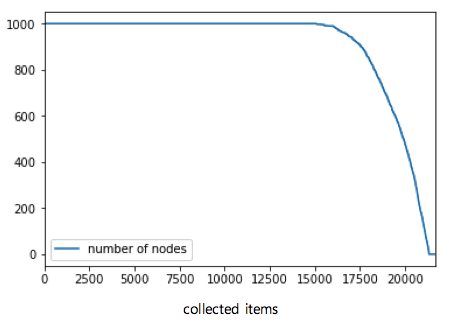
\includegraphics[width=0.7\columnwidth]{figs/figure_06_nr.png}
    \caption{Number of IPs reduced by detection}
    \label{fig:my_label}
\end{figure}

This is based on NASA traffic data in 1995, and can be applied to more or less crawler sets depending on the number of items the site has or the length of the long tail.
False positives occurred in 8 out of 6 matching data and 6 IPs were recognized as crawler nodes except duplicate detection. The number of requests generated per month for each IP is as follows.


\begin{table}
  \caption{IP and domains generated requests}
  \label{tab:freq}
  \begin{tabular}{ccl}
    \toprule
    IP or domain&Port\\
    \midrule
    156.80.168.122 & 117\\
    163.205.180.17 & 564\\
    dwkm206.usa1.com & 167\\
    jalisco.engr.ucdavis.edu & 424\\
    jbiagioni.npt.nuwc.navy.mil & 2124\\
    sputnix.cas.und.nodak.edu & 101\\
  \bottomrule
\end{tabular}
\end{table}


156.80.168.122 and sputnix.cas.und.nodak.edu, which generated relatively few requests, were detected as crawler nodes because the requests of these IPs were concentrated on a certain date, 29.7\% of them were in the long-tail area Of the respondents.

\end{enumerate}



%
% CONCLUSION
%
\section{CONCLUSION}
In this paper, we introduce a node reducing method that identifies the IP set of distributed crawlers and gradually reduces IP by using the property that web traffic follows the power law.
The node reducing scheme has shown a very low level of false positives against distributed crawlers using multiple IPs, effectively identifying crawler sets.



%
% FUTURE WORKS
%
\section{FUTURE WORKS}
Web traffic generally tends to generate traffic bursts at certain times. [1] Although the experiment of this paper is based on actual traffic log, since the time point of the data used in the experiment is one month, it does not include cases where a new item is added or an issue occurs and a traffic burst occurs.
In order to apply the results of this paper more securely to actual services, it is necessary to study whether the item movement level and threshold value of long-tail area can be maintained based on actual traffic data for traffic burst occurrence cases.



%
% REFERENCES
%
\section{REFERENCES}
[1]	M.V Simkin and V.P. Roychowdhury, “A theory of web traffic” https://arxiv.org/pdf/0711.1235.pdf
\newline[2] Density Estimation for Statistics and Data Analysis
\newline[3] Explaining World Wide Web Traffic Self-Similarity
\newline[4] Research on Detection Algorithm of WEB Crawler
\newline[5] Design and Implementation of Scalable, Fully Distributed Web Crawler for a Web Search Engine
\newline[6] Design and Implementation of a Distributed Crawler and Filtering Processor
\newline[7] URL Assignment Algorithm of Crawler in Distributed System Based on Hash
\newline[8] Design and Implementation of a High-Performance Distributed Web Crawler
\newline[9] Feature evaluation for web crawler detection with data mining techniques
\newline[10] Crawler Detection: A Bayesian Approach
\newline[11] Real-time Web Crawler Detection
[12] An investigation of web crawler behavior: characterization and metrics


% Bibliography
\bibliographystyle{ACM-Reference-Format}
\bibliography{sambib}




\end{document}
